% первая глава
\part{Изучение предметной области и анализ существующих подобных программных продуктов}

\section{Семейный бюджет с точки зрения экономики}

Бюджет в переводе с английского означает роспись денежных доходов и
расходов на определенный срок. Применительно к семейной экономике главный смысл бюджета заключается в не превышении расходов над доходами
за определенный промежуток времени при условии удовлетворения необходимых потребностей.
Количественный бюджет семьи определяет ряд факторов: численность
семьи, наличие в ней работающих; пенсионеров, стипендиатов и иждивенцев; размер заработной платы; величина пенсий, стипендий, пособий; наличие личного транспорта, подсобного хозяйства, проживание в городской или
сельской местности; национальные особенности.
Для того чтобы эффективно использовать свои доходы, семья должна правильно составить свой бюджет, тщательно продумать покупки и делать сбережения для достижения своих целей. Для составления семейного бюджета
необходимо подготовить список всех источников доходов каждого члена семьи. Это зарплата, социальные пособия и проценты на сбережения. В статье
расходов нужно перечислить все, за что надо заплатить в течение месяца:
квартплата и услуги, питание, проезд, уплата налогов и взносов. В планируемые расходы так же включаются и сбережения на будущее.
Если доходы равны расходам, то это сбалансированный бюджет. Если
предполагаемые расходы превышают доходы, то этот бюджет имеет дефицит. Бюджет, в котором доходы превышают расходы, будет иметь избыток.
Если расходы превышают доход, необходимо исключить из планов лишние
покупки, чтобы сбалансировать бюджет.

\section{Источники доходов и статьи расходов}

\subsection{Доходы}

\textbf{Cемья} - это объединение людей, которое основано на браке или кровном родстве и связано общим бытом, семейными доходами и взаимной ответственностью.

\textbf{Семейный доход} - это денежные средства, которые члены семьи получают
от посторонних лиц или организаций и могут использовать для оплаты собственных расходов. Все семейные доходы подразделяются на 2 вида:
денежные и натуральные. Основными денежными доходами семьи обычно
являются следующие 4 группы доходов:
\begin{enumerate}
\item Оплата труда членов семьи (заработная плата);
\item Поступление из общественных фондов потребления (часть доходов семья получает в виде бесплатных услуг, денежных выплат, льгот);
\item Прочие (случайные) доходы (вознаграждения, наследство, подарки);
\item Доходы от домохозяйственной и предпринимательской деятельности.
\end{enumerate}
Натуральные доходы семьи могут быть в виде различной продукции собственного домохозяйства, готовой продукции предприятий выдаваемой ими
в счёт заработной платы, а также различные материально-вещественные ценности, получаемые членами семьи в порядке пособия, пожертвования, дарения и т.п. Натуральные доходы при их суммировании с денежными доходами
оцениваются по средним рыночным ценам в данном регионе на дату получения этих натуральных доходов.
Все суммированные денежные и натуральные доходы подразделяются на
несколько видов в зависимости от степени полноты их исчисления. Наиболее
полными являются совокупные доходы семьи, представляющие собой сумму всех денежных и натуральных доходов всех членов семьи. Все денежные
и натуральные доходы семьи, которые подлежат налогообложению, называются совокупными налогооблагаемыми доходами. А совокупные доходы за
вычетом всех налогов и обязательных платежей составляют располагаемые
или чистые доходы, поступающие в полное распоряжение семьи.

\subsection{Расходы}
Семейные расходы можно разделить на 4 группы:
\begin{enumerate}
\item Обязательные (жилищно-коммунальные услуги, телефон, медикаменты,
налоги);
Эта группа расходов имеет неприятное свойство - накапливаться в виде
долга, если они не производятся своевременно.
\item Текущие (продукты питания, транспорт, промышленные товары);
\item Периодические (досуг, развлечения); Эти расходы особенны тем, что носят вероятностный характер. Они могут быть в определ нном месяце, квартале, но могут и не появиться,
\item Единовременные расходы (приобретение значительных по стоимости вещей).
Производятся несколько раз в несколько лет.
\end{enumerate}

Кроме того, в течение года могут быть и одноразовые затраты - взносы в
общественные фонды, сезонные закупки, подписка, оплата пут вок в санаторий и т. п.
Так же в условиях продолжительных периодов анализа формирования семейного бюджета, нельзя не учитывать влияние на экономику семей столь
мощного процесса, как инфляция.

\section{Составление плана доходов и расходов семьи}
Для обеспечения стабильного материального положения семьи, а тем более для повышения ее благосостояния необходимо планирование семейного
бюджета.
Первой предпосылкой и обязательным условием планирования семейного
бюджета является учет доходов и расходов семьи.
Планирование семейного бюджета - это прогнозирование изменений доходов и расходов семьи на предстоящий период, определение организационноэкономических и финансовых мер по сбалансированности доходов и расходов,
получению и эффективному использованию семейных накоплений.
Планирование семейного бюджета осуществляется в следующем порядке:
\begin{enumerate}
\item Прогнозирование доходов семьи;
\item Прогнозирование расходов семьи;
\item Сопоставление предстоящих доходов и расходов;
То есть их балансировка и регулирование посредством поиска дополнительных источников доходов и определения мер по сокращению расходов семьи.
\item определение и распределение ожидаемых семейных накоплений.
\end{enumerate}
Чтобы составить проект бюджета семьи, нужно ответить на три вопроса:
\begin{enumerate}
\item Сколько денег имеем;
\item Как их истратить, чтобы удовлетворить насущные потребности не влезая в долги;
\item Как распределить покупки во времени, увязав их с доходами и возможностями,предоставляемыми торговлей и предприятиями службы быта.
\end{enumerate}
ак и в экономике промышленных предприятий, в семейной экономике
должно быть годовое, месячное и недельно-суточное планирование. Исходным моментом составления бюджета семьи является оценка по доходной части во времени - на месяц, на год. Это заработная плата членов семьи плюс
выплаты из общественных фондов потребления. Желательно оценить возможные изменения составных частей дохода в планируемом периоде. Например, премиальные доплаты могут изменяться помесячно, поквартально, и их
при годовом планировании следует включать в расчет на среднем уровне по
прошлым периодам. Нужно оценить изменения в заработной плате в связи с возможностями повышения квалификации, повышением в должностной
иерархии или смену работы, которая приведет либо к прибавке, либо к уменьшению доходов. Также нужно учесть и возможное снижение доходов семьи
(например, переход одного из членов семьи на пенсию, рождение ребенка и
т. д.).
Доходы целесообразно учитывать ежемесячно, а сезонные (например, доходы от подсобного хозяйства) или единовременные - в расчете на квартал,
полугодие, год.
% второй раздел - файл part2.tex

\section{Методики учета семейного бюджета}

\subsection{Где вести учет семейного бюджета}

\subsubsection{Тетрадь или амбарная книга}
Несомненно, что для вычислений, связанных с учетом личных финансов,
было бы удобно воспользоваться компьютером и вести в нем все записи, однако если такой возможности нет, то можно завести тетрадь или амбарную
книгу. В самом простом обобщенном случае рекомендуется разбить лист на
три графы:
\begin{table}[H]
	\caption{Пример теблицы для учета семейного бюджета}
	\label{tab:t1}
	\begin{center}
		\begin{tabular}{|r|p{5.5cm}|p{2.5cm}|}
			\hline 
			Доход & Расход & Итого \\ 
			\hline 
			&  &  \\ 
			\hline 
		\end{tabular} 
	\end{center}
\end{table}

Графы Расход и Доход будут отражать соответствующее движение
денег вашего кошелька, а графа Итого нужна для того, чтобы сверять цифры на бумаге с количеством денег в карманах. Как ни странно, они должны
совпадать.
Такой подход в целом приемлем для одного человека, он даже позволит
отследить и выявить необязательные расходы, которые впоследствии можно
уменьшить или вовсе убрать. Однако в таком виде о какой-либо наглядности
и систематизации говорить не приходится. Тем более в рамках рассмотрения
бюджета семьи. Ведь, как уже говорилось в предыдущей части, семейный
бюджет охватывает множество составляющих.
Для повышения наглядности и хоть какой-то систематизации доходов и
расходов, приведенную табличку необходимо разбавитьї дополнительными
колонками группируя разные виды расходов в соответствии реально имеющимся.
Например, в первую колонку можно записывать коммунальные платежи,
свет, интернет или аренду. Во второй колонке записывать лишь траты на
продукты питания, в третьей личные расходы, в четвертой расходы на развлечения и в пятой непредвиденные расходы.
Естественно, существующую таблицу нужно модернизировать под себя и
вероятно кто-то посчитает нужным добавить колонки по бытовой химии, уходу за кошкой, ребенком, родителями и т.д.
Эти расширения, в конце концов, приведут к тому, что таблица попросту
перестанет умещаться даже в амбарную книгу. И в этом случае на помощь
приходят компьютерные программные средства.

\subsubsection{Электронные таблицы}
Более продвинутый путь, приступить к ведению семейного бюджета при
помощи электронной таблицы (Excel, Google Docs и т.п.), где уже даже имеются основные формулы для анализа бюджета. По сути, вам остается лишь
выбрать и применить их к своим данным. Но и тут есть путь проще.
Дело в том, что на сегодняшний день существует множество специальных
шаблонов для электронных таблиц, в которых уже учтены некоторые наиболее популярные поля и необходимые для расчетов формулы.
\subsubsection{Специализированные программы}
Кроме шаблонов для табличных редакторов, в сети интернет предлагается
масса специальных программ для ведения учета и планирования семейного
бюджета.
Они позволяют автоматизировать большую часть работы, что значительно
упрощает процесс ведения домашних финансов.
Помимо того, эти программы, как правило, имеют массу вспомогательных функций, которые позволяют выявить слабые и сильные стороны вашего отношения с деньгами, помогут явно обратить внимание на, казалось бы,
очевидные, вещи, но почему-то не используемые в повседневной жизни. По
сути, программы для ведения семейного бюджета значительно облегчают и
помогают создать целостную картину наших взаимоотношений с финансами.
\section{Существующие решения}
\subsection{GnuCash}

\textbf{Тип}: персональная бухгалтерская система\\
\textbf{Автор}: Robin Clark - X-Accountant,
Gnumatic (Linas Veptas)\\
\textbf{Разработчики}: GnuCash development team\\
\textbf{Язык программирования}: C, Scheme и Java\\
\textbf{Интерфейс}: 	GTK+\\
\textbf{Операционная система}: GNU, GNU/Linux, FreeBSD, macOS, Microsoft Windows и Android\\
\textbf{Первый выпуск}: 1998\\
\textbf{Лицензия}: 	GNU GPL 2\\

\begin{figure}[H]
	\centering
	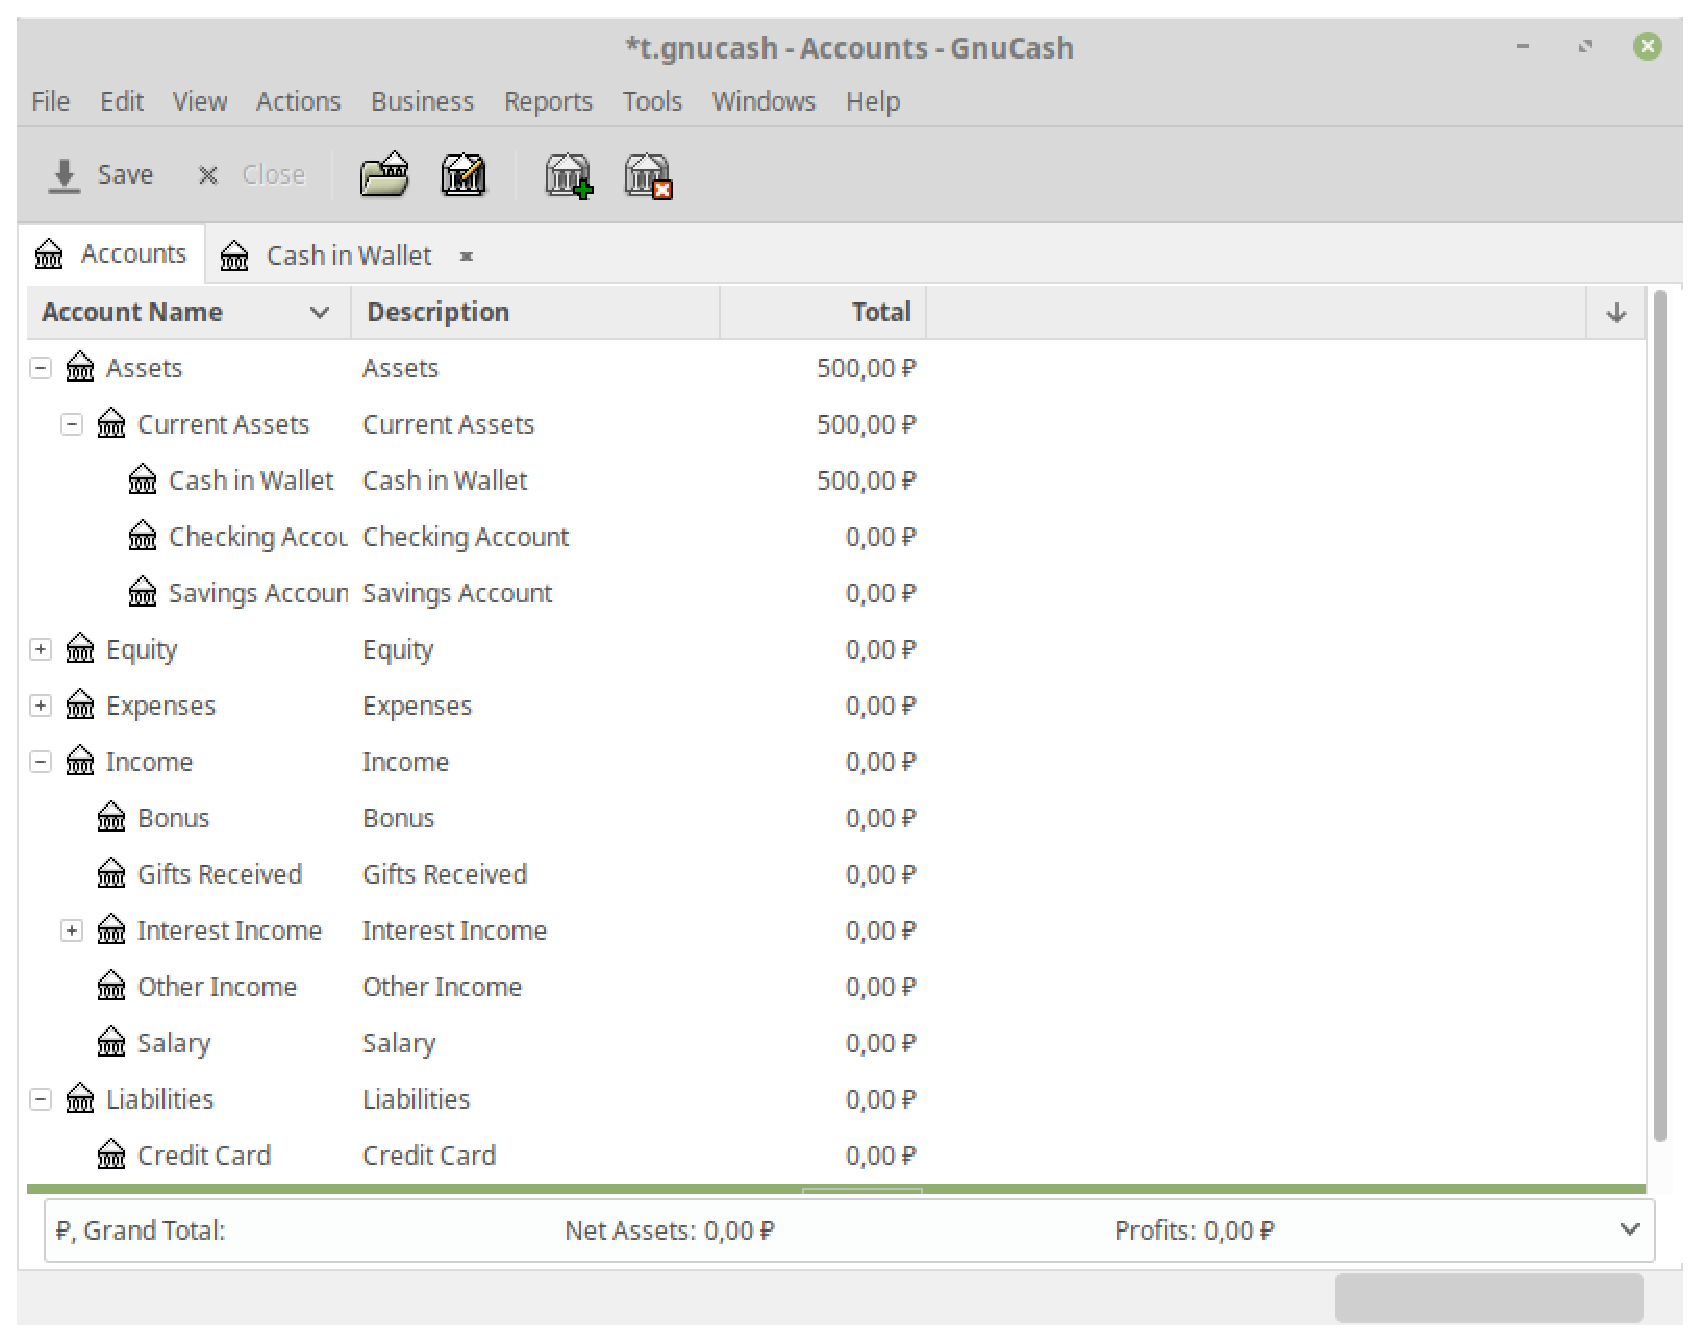
\includegraphics[width=1\linewidth]{pics/GnuCash.eps}
	\caption{Интерфейс GnuCash}
	\label{fig:GnuCash}
\end{figure}

Один из самых известных проектов в мире персональных финансов. Разрабатывается с 1997 года как продукт с отрытым исходным кодом.\\

При переходе на эту программу с других проектов могут возникнуть сложности, т.к. принципы работы GnuCash основаны на системе с двойной записью, характерно скорее для профессиональных платформ бухгалтерского учета. Однако хорошо организованная документация на разных языках (русский есть) и хорошая поддержка помогут быстро разобраться.\\

Почти все свойства программы в сравнении с другими продуктами заслуживают максимальной оценки. Программа продуманна в мельчайших деталях. Способна учитывать различные типы инвестиций, включая драгоценные металлы, ценные бумаги, котирующиеся на наиболее известных биржах (ММВБ нет). Алгоритмизация учета кредитов и других видов долга также на высоком уровне. Среди всех проектов из нашего обзора GnuCash имеет саму продуманную и гибкую систему анализа данных с многочисленными настройками (некоторые из функций анализа есть и в мобильном приложении).\\

Среди слабых мест – ее несколько устаревший интерфейс. Однако он вполне удобен и функционален. При знакомстве с GnuCash становится понятным, откуда многие другие проекты «позаимствовали» основные идеи.\\

Другим очевидным минусом являются минималистичные возможности по синхронизации данных. Предусмотрена только полуручная синхронизация через Google Drive и DropBox, что подходит не для всех. Из этого минуса вытекает и следующий – многопользовательского режима в программе просто нет.\\
Функциональные возможности:\\
\begin{enumerate}
	\item Графический интерфейс пользователя
	\item Стандартная двойная запись для ведения бухгалтерского учёта
	\item Транзакции по расписанию
	\item Учёт кредитных платежей
	\item Построение отчётов и графиков
	\item Поддержка бухгалтерского учёта для малых предприятий
	\item Импорт файлов данных из других финансовых систем OFX, QIF
	\item (Ограниченная) поддержка многопользовательского интерфейса баз данных SQL
	\item Многовалютный учёт
	\item Работа с портфелем акций и паями паевых инвестиционных фондов
	\item Получение данных об акциях и паях через интернет
	\item Финансовый калькулятор
\end{enumerate}
\textbf{Плюс}: Распространяется бесплатно, предусмотрены многие профессиональные функции бухгалтерского учета, возможность ведения управленческого учета для малого бизнеса, постоянное развитие проекта.\\
\textbf{Минус}:Несколько сложна в освоении, принципы работы программы значительно отличаются от большинства других проектов, несколько устаревший интерфейс, отсутствие полноценной синхронизации и многопользовательских возможностей.\\
\pagebreak

\subsection{Streege}
\begin{figure}[H]
	\centering
	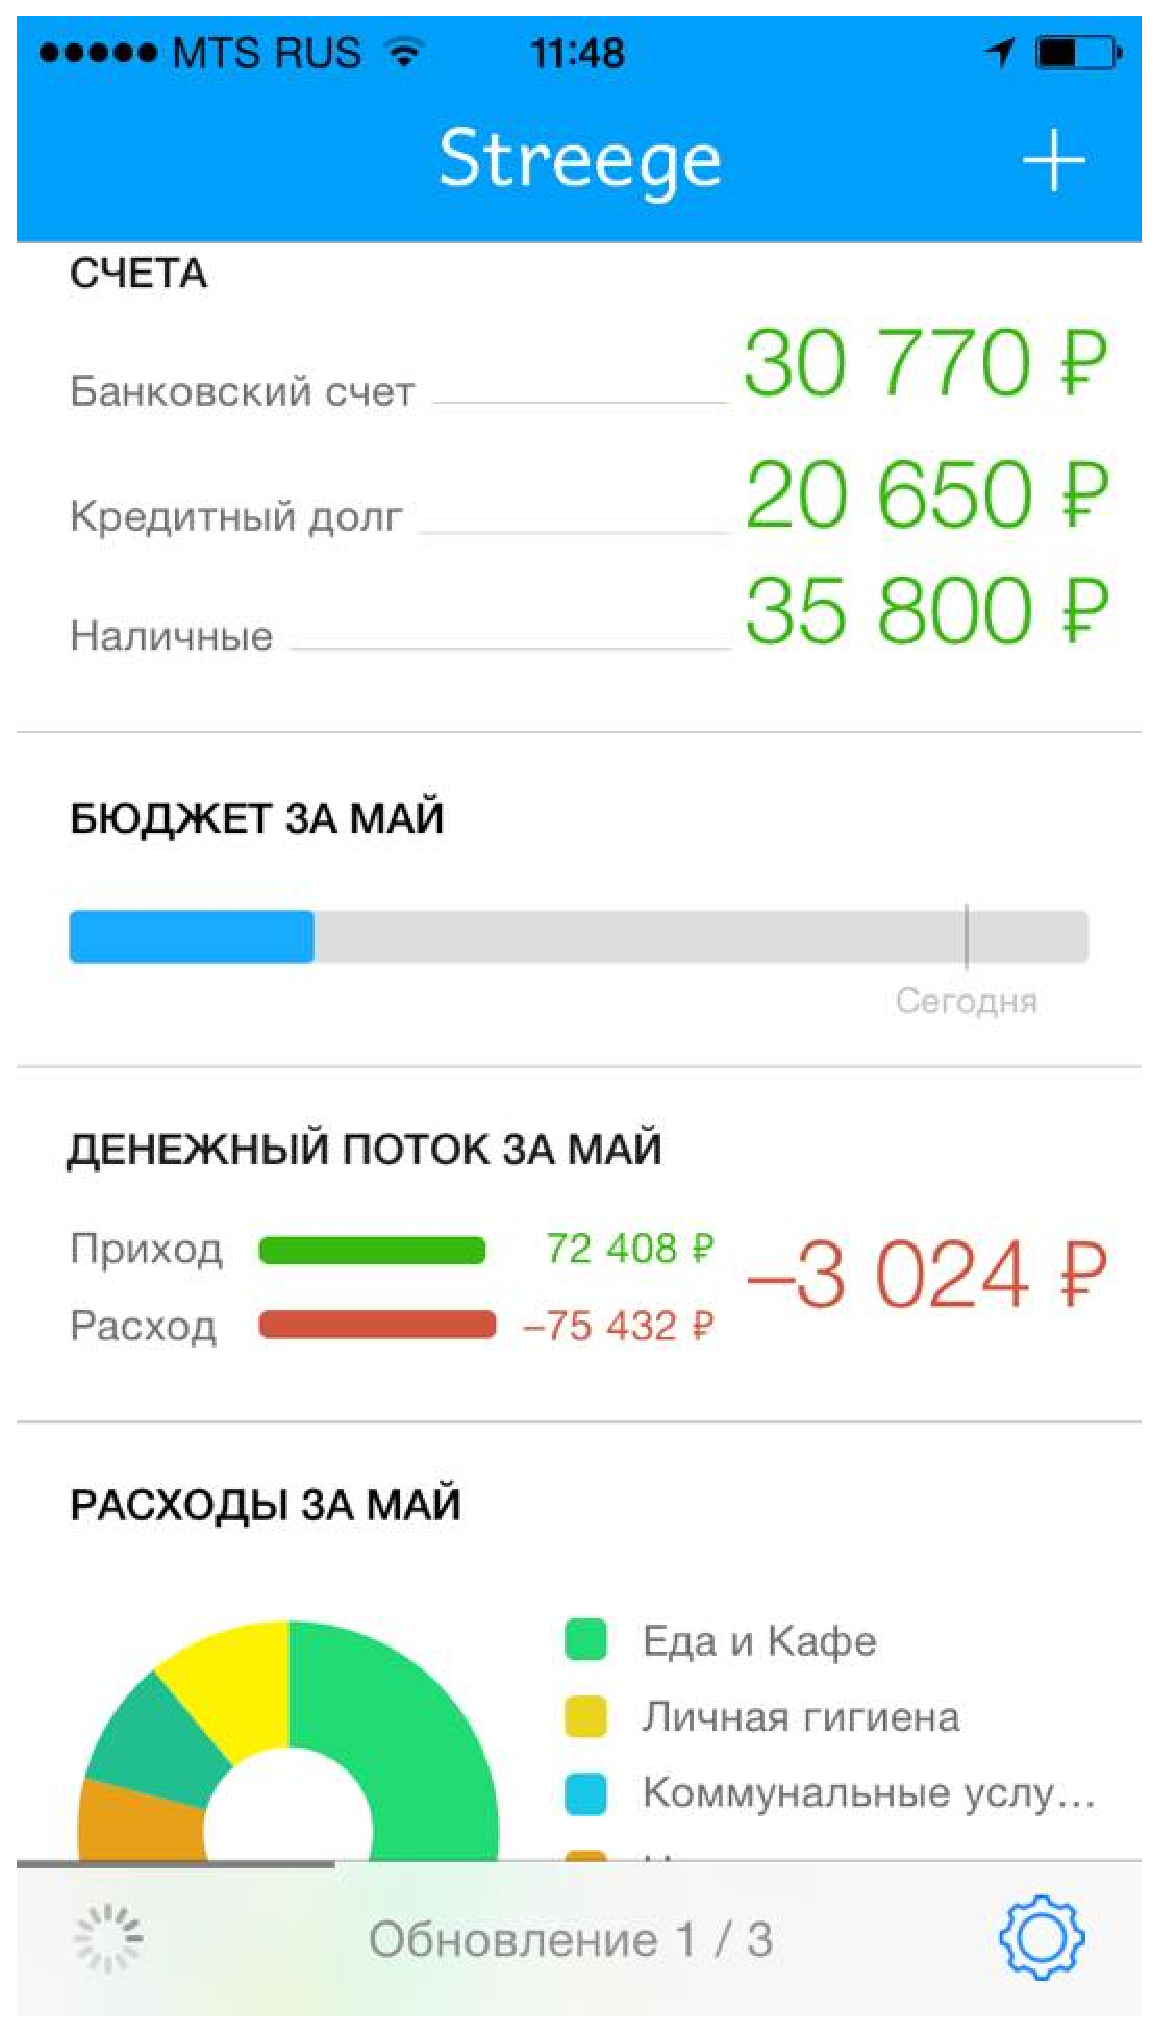
\includegraphics[width=0.7\linewidth]{pics/Streege.eps}
	\caption{Интерфейс Streege}
	\label{fig:Streege}
\end{figure}
Проект запущен авторами CashOrganizer в 2014 году. Это первая на российском рынке программа, которая умеет в автоматическом режиме (без использования СМС и email) синхронизироваться с банками и загружать данные о транзакциях и балансах счетов. Категории платежей так же присваиваются автоматически. Впрочем, все данные платежа после загрузки могут быть отредактированы вручную.\\

Концепция проекта очень удобна для повседневного использования. «Руками» нужно вносить только транзакции из наличных. В перечне уже 177 основных российских банков. Для синхронизации с некоторыми из них (Сбербанк, ТКС и другие) требуется вводить код, высылаемый по смс. Другие (Авангард, Альфа Банк и др.) работают без всяких подтверждений. Но даже введение раз в несколько дней кода из СМС особых проблем не вызывает.\\

Пока в проекте нет онлайн синхронизации, нет сплита транзакций и еще некоторых мелочей. Но проект развивается довольно быстро. Надеемся на исправления всех недочетов.\\

Кроме того, надо конечно понимать, что как у всех проектов, нацеленных на мобильные платформы, возможности для анализа данных и другие продвинутые функций здесь будут ограничены по определению. К сожалению информации по этому продукту очень немного\\
\textbf{Плюс}: Автоматическая система загрузки транзакций из банков. Автоматическое присвоение категорий транзакциям.
\\
\textbf{Минус}:Нет синхронизации.\\
\pagebreak

\subsection{MoneyWiz}
\begin{figure}[H]
	\centering
	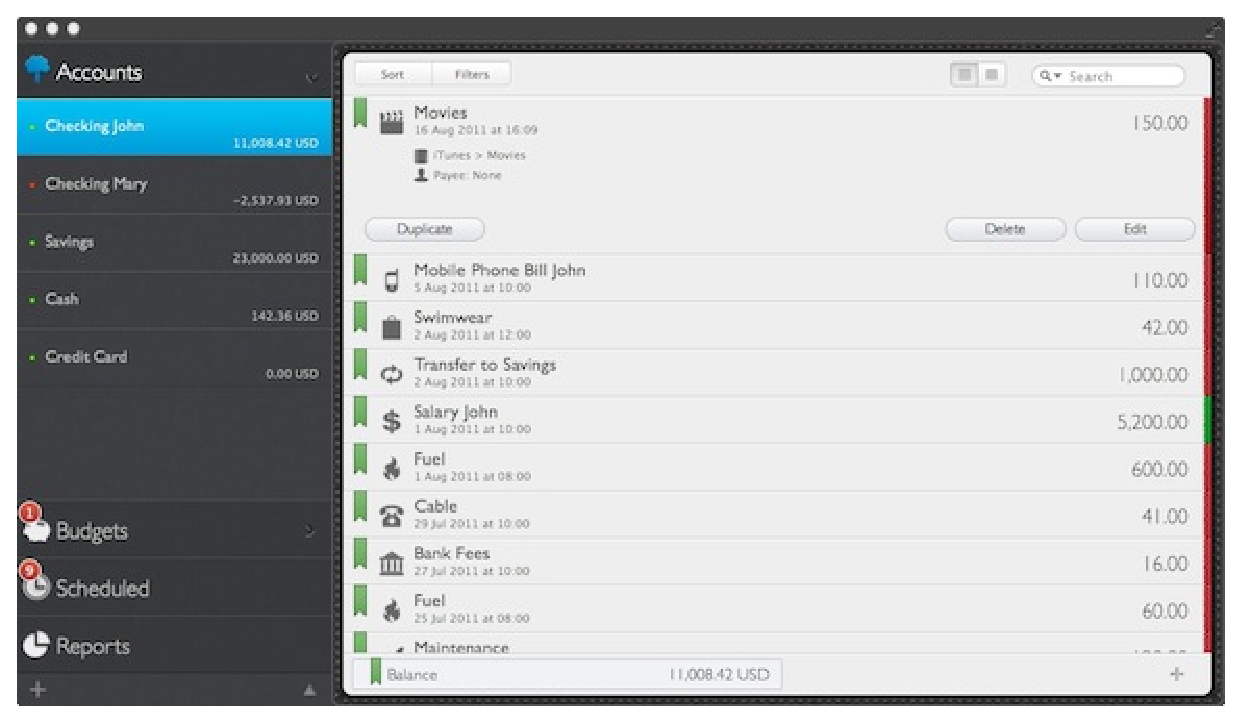
\includegraphics[width=1\linewidth]{pics/MoneyWiz.eps}
	\caption{Интерфейс MoneyWiz}
	\label{fig:MoneyWiz}
\end{figure}
Проект существует с 2011 года и был разработан с прицелом на iPad. MoneyWiz и сейчас остается сервисом с наибольшим количеством возможностей для пользователей устройств Apple. Только для MacOS есть десктоп версия. Хотя на сайте проекта уже анонсирована версия под Windows.\\

Из полезных и оригинальных функций – возможность настройки представления окна ввода транзакций. Это окно используется чаще всего в любой программе, и возможность его настройки «под себя» сильно упрощает жизнь.\\

В проекте много функций, которые сделаны специально для пользователей Apple. В iOS версии есть поддержка Touch ID и экспорта через AirDrop. Есть специальная версия программы для Apple Watch.\\

Удивительно хорошей проработкой, особенно для мобильного приложения, порадовали отчеты с довольно удобными настройками.\\

Из грустного – главный плюс программы, а именно автоматическая синхронизация транзакций с банками, работает пока не всегда корректно. Команда сайта rostber.ru протестировала работу с четырьмя российскими банками. Банк Авангард – всё работает нормально. Альфа банк – настроить не получилось. Сбербанк – транзакции загружаются нормально, но баланс отображается неправильно. Тинькофф банк – транзакции загружаются нормально, но баланс отображается неправильно. Пока такие результаты синхронизации вряд ли можно считать приемлемыми, особенно для платного сервиса (примерно 300 руб в месяц). Хотя не приходится сомневаться, что по примеру проекта Стриж, сервис удастся довести до нормальных результатов. Пока MoneyWiz – это единственный проект, где синхронизация транзакций заявлена как для зарубежных и российских банков. Всего проект поддерживает синхронизацию с 15 тыс. банками из 43 стран.\\

Другим явным недостатком является отсутствие колонки (или итога по дням) для баланса счета в перечне транзакций. Во всех продвинутых программах этого уровня балансы ужа давно интегрированы и значительно упрощают жизнь.\\

Странным показалось, что при возможности формирования неограниченного числа бюджетов нельзя включать в них доходные категории (только расходы).\\

MoneyWiz известен, как проект одним из первых в мире (если не первый) проектов в области личных финансов, запустивший синхронизацию данных через облачный сервис. Это случилось в 2011 году. Жаль, что с тех пор мало что изменилось. Синхронизация данных возможна только через непонятный SYNCbits, где необходимо создать учетную запись.\\

Описание функций программ есть только на сайте и только на английском. Каких-либо обучающих материалов не предусмотрено.\\

\textbf{Плюс}: Автоматическая синхронизация транзакций с российскими и западными банками.
\\
\textbf{Минус}:Ошибки в синхронизации транзакций с банками.\\
\textbf{Минус}:Сравнительно высокая стоимость.\\
\pagebreak



